\documentclass{article}
\usepackage{amsmath}
\usepackage{amssymb}
\usepackage{parallel}
\usepackage[most]{tcolorbox}
\usepackage{amsthm}
\usepackage[a4paper,
top=1.5cm,
bottom=1.5cm,
left=1.8cm,
right=1.8cm,
heightrounded]
{geometry}
\renewcommand{\arraystretch}{2.5}
\usepackage{subfig}

\title{QF 620 \protect \\ Stochastic Modelling in Finance\\
\textbf{Project Report}}

\date{}

\begin{document}

\section{Delta Hedging} 

\noindent \textbf{\textit{\underline{Assumptions of the results}}}\\ \\
With the following assumptions of the options parameters below:\\ 

\begin{center}
$S_0 = \$100 ,r = 0.05, \sigma = 0.2, K = \$100$ 
\end{center} 

\noindent We have managed to run a total of 50,000 paths to simulate discrete delta hedging and the following is a chart of the paths taken in the one period, in which the price varies from 80-130.\\ \\

\begin{center}
	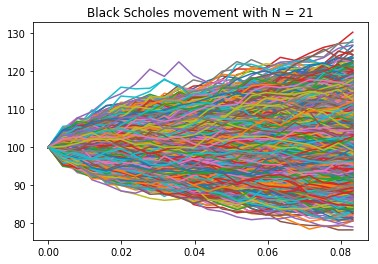
\includegraphics{./images/BS_stock_paths.jpg}
\end{center}

\begin{center}
	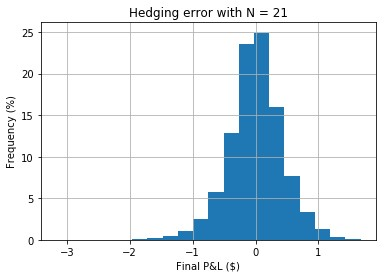
\includegraphics[width=0.5\textwidth]{./images/21_steps_D_Hedge.jpg}%
	\includegraphics[width=0.5\textwidth]{./images/84_steps_D_Hedge.jpg}
\end{center}

\begin{center}
\begin{tabular}{|c|c|}
	\hline
	\textbf{Mean P\&L}& \textbf{Standard Deviation}\\
	\hline
	0.003 & 0.428
	\\
	\hline
\end{tabular}
\qquad\qquad\qquad
\begin{tabular}{|c|c|}
	\hline
	\textbf{Mean P\&L}& \textbf{Standard Deviation}\\
	\hline
	0.000 & 0.218
	\\
	\hline
\end{tabular}
\end{center}

\newpage

\noindent\textbf{\textit{\underline{Discussion of the results }}}\\ \\

\noindent Next, we have conducted a test whereby we carried out delta-hedging at every timestep, N=21,84, and the following charts show the results of the delta hedge. As we can witness in the results, the expected value of the final PNL seems to be close to each other but the standard deviation of N=21 is almost twice of N=84. This thus shows that there is a large variation in the pnl when we hedge at a much fewer frequency, which would be disastrous if there were to be spikes in the underlying prices. In addition, the following chart display a negative skewness (i.e. fat tail towards the left), and this thus shows that there’s a slim probability whereby one can end up extreme end of the chart which would be highly undesirable for the hedger. \\ \\


\noindent \textbf{\textit{\underline{Qualitative assessment of the results}}} \\ \\

\noindent The assumption of the Black-Scholes replication strategy is to delta-hedge continuously till the option’s maturity but this is not made possible due to the real-world limitations. Therefore, that can only suggest discrete delta hedging in which one can short or long the underlying asset to remain delta-neutral at each time step. However, this still has its own pitfalls which will be discussed below. \\ \\

\noindent In the case of discrete delta hedging, we would only be sampling the underlying prices of the stock intermittently, i.e. at per time step of N = 21/84 steps, and the results would therefore not be a true indicative of the underlying volatility. Even with a known constant volatility and no spikes to the underlying asset price, the measured volatility across some paths would still deviate away from the 20\% constant volatility mark due to statistical fluctuations.  This therefore introduces replication error as the delta-hedge uses a constant volatility of 20\% that might not be the true delta to be hedged. This is highly undesirable as this leaves us to have a delta exposure which might lead to favour or disfavour to the PNL.  In addition to that, we can also observe that the PNL has a negative skewness which might expose us to severe downside risk due to our delta exposure. \\ \\

\noindent Therefore, in order to reduce potential downside risk due to the replication error and negative skewness, we can increase the delta-hedging frequency in order to minimize the standard deviation of our PNL. As shown in the results, the standard deviation was almost halved once the delta hedge is performed at 4 times per days as compared to daily. Despite the existence of replication error still, increase in the hedging frequency allows us to match much closely to the true volatility of the underlying price which can help reduce large undesirable losses in our trading P\&L. \\ \\

\noindent In conclusion, discrete delta hedging would lead to potential losses due to replication error, and one should look to increase the hedging frequency in order to reduce the potential downside risk. In addition to that, one should also incorporate other important factors such as possibility of underlying prices spikes, changes in the volatility, and transaction costs, in order to create a much realistic delta hedging strategy. 

\end{document}